\documentclass{book} 
% \usepackage{classicthesis}
\usepackage{thesis}
% \setstretch{1.05} % 1.1 line spacing

\raggedbottom
\begin{document}
\fontsize{11.5pt}{14pt}\selectfont
 
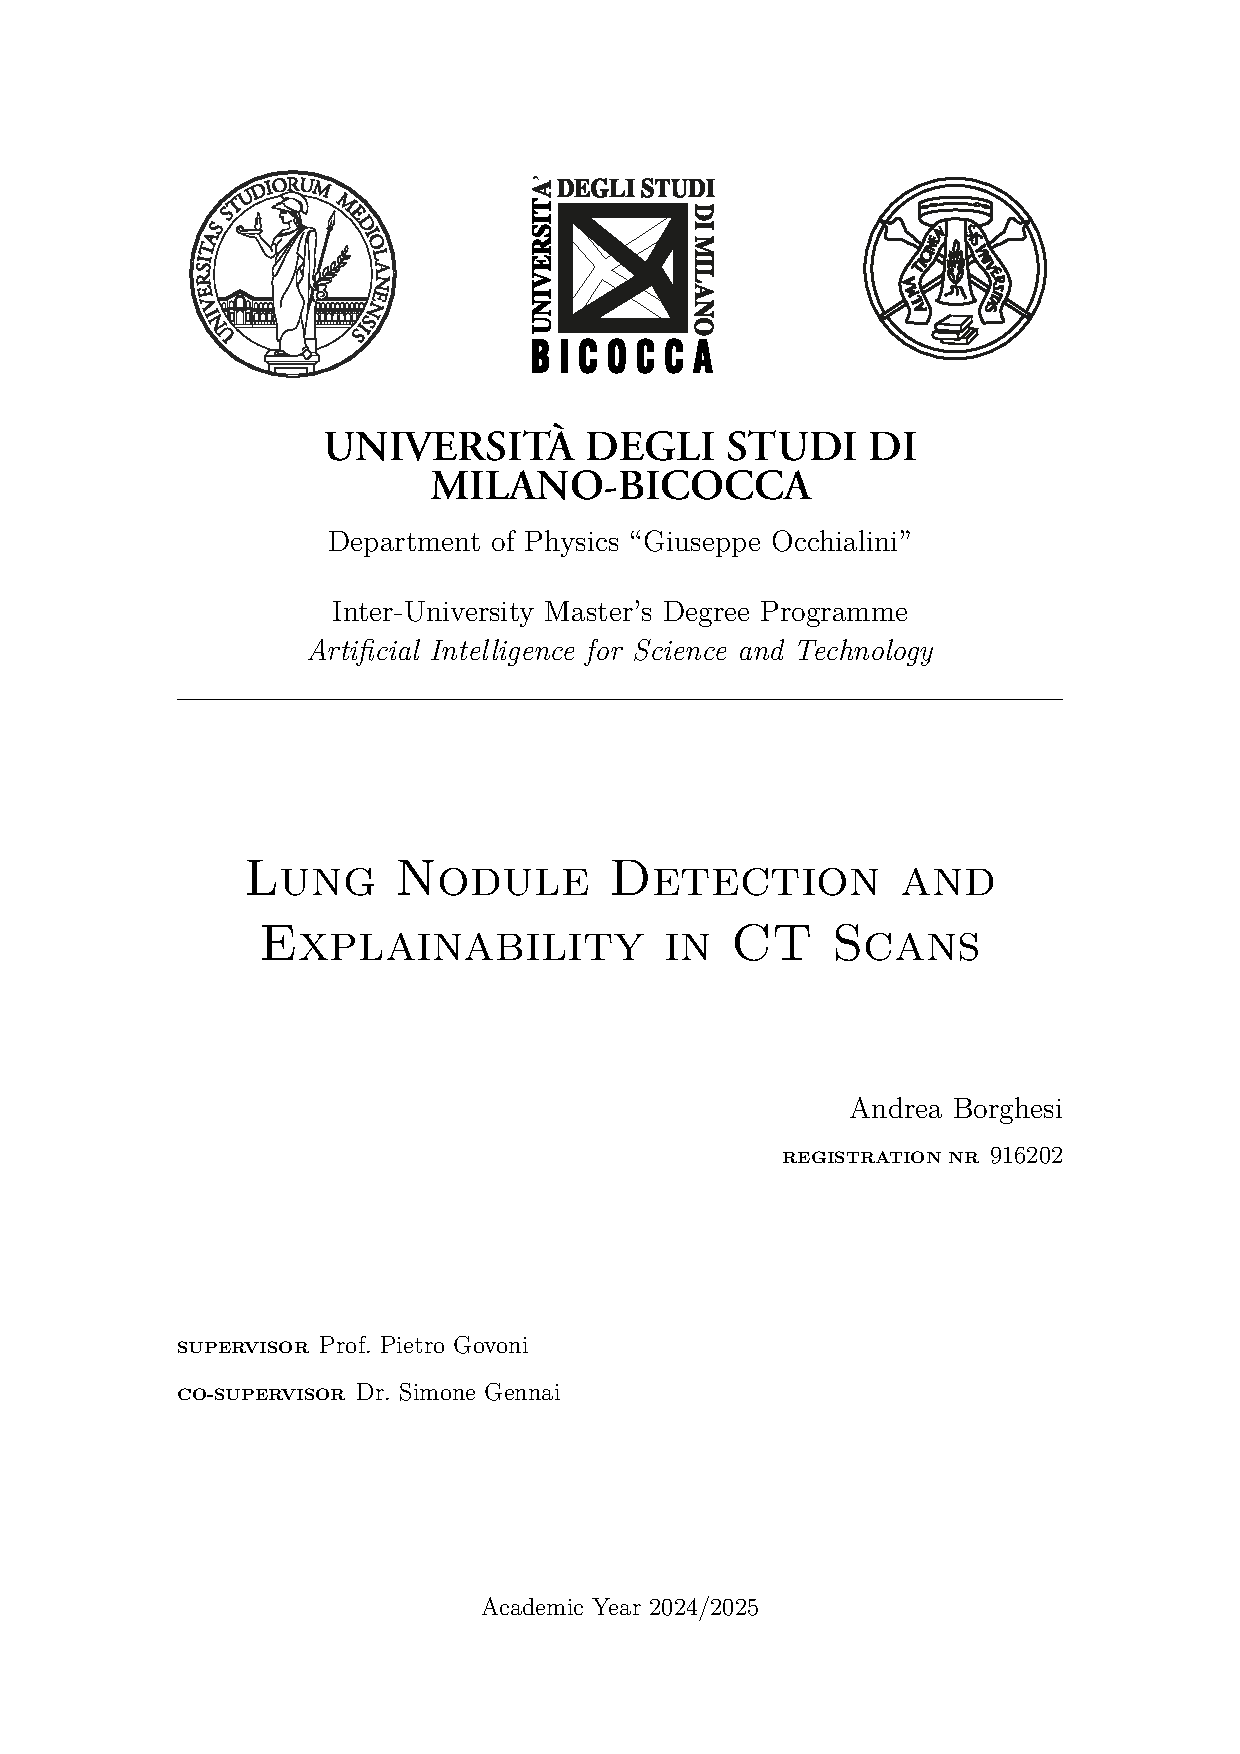
\includepdf{thesistitlepage/titlepage.pdf}
\cleardoublepage
\pagenumbering{gobble}
\chapter*{Abstract}
    The early detection of pulmonary nodules through Computed Tomography (CT) screening is crucial for improving patient outcomes in lung cancer, yet the manual review process is a significant burden on radiologists. While Deep Learning models offer a promising solution, state-of-the-art 3D approaches are often computationally expensive and lack transparency, hindering their widespread adoption.

    This thesis addresses these challenges by developing and evaluating a lightweight, 2D-based pipeline for the detection and explainability of lung nodules in CT scans. The core of the pipeline is a Faster R-CNN architecture, systematically evaluated with various efficient backbones. To mitigate the loss of volumetric information inherent in a 2D approach, a 2.5D input representation that stacks adjacent slices is employed. A secondary classification model is also developed to characterize detected nodules as benign or malignant.

    A central contribution of this work lies in adapting and quantitatively evaluating gradient-free Class Activation Map (CAM) methods for the task of object detection. A custom similarity metric was designed to make Score-CAM and Smoothed Score-CAM (SS-CAM) compatible with the structured outputs of the detector. The faithfulness of these methods, alongside Eigen-CAM, was objectively measured using a novel ``Inverse Distance Game" protocol.

    The results demonstrate that the lightweight detection pipeline establishes a strong performance baseline, with the EfficientNetV2-S backbone proving most effective. For explainability, the quantitative evaluation reveals that Eigen-CAM provides significantly more faithful and well-localized explanations than the adapted Score-CAM and SS-CAM variants, while being orders of magnitude more computationally efficient.

    Ultimately, this research validates the feasibility of computationally accessible 2D methods for lung nodile detection and contributes a framework for adapting and evaluating explainability techniques in object detection. The findings identify Eigen-CAM as a practical and effective method for providing trustworthy visual explanations in this medical imaging context.

\frontmatter
\cleardoublepage
\tableofcontents

\mainmatter

\chapter{Introduction}
\label{ch:introduction}

\section{Problem Statement and Motivation}

Lung cancer remains one of the leading causes of cancer-related mortality worldwide, with early detection being crucial for improving patient outcomes and survival rates. Computed Tomography (CT) screening programs, such as the National Lung Screening Trial (NLST), have demonstrated the potential to reduce lung cancer mortality through early identification of pulmonary nodules \cite{aberle2011reduced, de2020reduced}. However, the manual interpretation of CT scans is a time-intensive process that places significant burden on radiologists, while also being subject to inter-observer variability and potential oversight of small or subtle lesions.

Radiologists are often required to review hundreds of slices per patient, sometimes across dozens of patients in a single day. Under such conditions, cognitive fatigue can accumulate, potentially leading to decreased diagnostic precision, delayed reading times, or even missed findings, especially for low-contrast or small nodules that may appear on only a few slices \cite{stec2018systematic, taylor2019fatigue}. This challenge is further amplified in high-volume screening programs, where maintaining consistent accuracy over long hours is difficult even for experienced professionals.

Artificial intelligence (AI) based detection tools have the potential to alleviate this strain by automatically flagging suspicious regions of interest, enabling radiologists to focus attention on the most relevant slices. Such systems do not replace human expertise but can act as a second reader, improving sensitivity to subtle findings, reducing oversight caused by fatigue, and providing explainable visual cues that support decision-making and increase trust in automated recommendations \cite{glikson2020human}. 
On this note, it is important to mention that it has been shown that the use of AI can instead increase fatigue to radiologists with higher workload if they have a low acceptance of AI \cite{liu2024artificial}. Regardless, the integration of AI tools into clinical workflows has been shown to enhance diagnostic accuracy  and efficiency, ultimately leading to better patient care and outcomes \cite{guermazi2022improving,huynh2020artificial}.

Nevertheless, existing AI solutions are often limited by computational demands and lack transparency in their predictions, motivating the need for efficient and explainable detection methods specifically tailored to lung nodule identification in CT scans.
This need is further reinforced by the recent European Union Artificial Intelligence Act, which establishes a regulatory framework that emphasizes transparency, accountability, and human oversight for AI systems—particularly in high-risk domains such as healthcare \cite{eu_ai_act}.

\section{Research Challenges}

Designing AI-based tools for lung nodule detection in CT scans involves navigating a complex landscape of technical and practical challenges that significantly limit the applicability of existing solutions in real-world clinical environments.

The most immediate challenge stems from the computational demands of state-of-the-art approaches. While three-dimensional convolutional neural networks can theoretically exploit the full volumetric context of CT scans to improve detection accuracy, their practical implementation reveals significant limitations. These models typically require substantial GPU memory, often exceeding 16GB, and demand extensive training times that can extend to days or weeks, even on high-end hardware such as A100 GPUs with 40GB of memory \cite{wu2018systematicanalysisstateoftheart3d}. While inference times for individual patient scans may be manageable, the development and iterative improvement of such models becomes prohibitively expensive and time-consuming. 
Such computational requirements create a fundamental mismatch with research development processes, where rapid experimentation and iteration are crucial for advancing the field, especially in small research groups with limited access to high-end hardware.
This computational constraint naturally leads to consideration of more efficient 2D approaches, which process individual CT slices rather than entire volumes. This approach significantly reduces memory requirements and training times, allowing for more agile development cycles, at the cost of losing correlations between slices that may be crucial for accurate nodule detection. Regardless, a 2D approach allows for better accessbility to healthcare professionals, as it can be run on standard laptops or workstations without the need for high-end GPUs.
Equally critical, yet often overlooked in the technical literature, is the challenge of explainability in object detection systems. The medical domain presents unique requirements for AI interpretability, driven by regulatory demands, clinical decision-making needs, and the fundamental requirement for physician trust and acceptance. However, most existing explainability methods were developed for image classification tasks \cite{selvaraju2019gradcam,chattopadhay_2018gradcam++,draelos2021hirescam,jiang2021layercam}, where the goal is to explain a single prediction score for an entire image. Object detection fundamentally differs in that as it produces structured outputs consisting of multiple bounding boxes, each with associated class probabilities and confidence scores.
This structural difference creates significant technical obstacles for applying standard explainability techniques.

\section{Research Questions and Objectives}
The challenges outlined in the previous section give rise to three primary research questions that guide this thesis:

\paragraph{RQ1: How can 2D object detection approaches achieve clinically relevant performance for lung nodule detection within computational constraints?}
This question addresses the fundamental trade-off between computational efficiency and detection performance. While 3D approaches theoretically offer superior performance by exploiting volumetric context, their computational demands make them impractical for many research and deployment scenarios. We investigate whether 2D slice-based detection can achieve acceptable performance levels while operating within the memory and processing constraints of standard hardware configurations.

\paragraph{RQ2: How can explainability techniques be adapted for the structured outputs of object detection models?}
Standard explainability techniques are designed for classification tasks with single prediction scores, but object detection produces complex structured outputs with multiple bounding boxes, confidence scores, and non-differentiable post-processing steps. This question explores how gradient-free Class Activation Map (CAM) methods can be modified to generate meaningful explanations for object detection predictions, addressing the technical challenges posed by structured outputs and non-differentiable operations.\bigskip

To address these research questions, this thesis pursues the following specific objectives:
\paragraph{O1: Develop a computationally efficient 2D object detection pipeline for lung nodule detection}
Implement and compare multiple object detection architectures and their variants.
Design preprocessing pipelines optimized for 2D slice-based analysis, including slice selection algorithms to maximize information content.
Achieve detection performance that demonstrates clinical viability while operating within 16GB GPU memory constraints.

\paragraph{O2: Adapt CAM methods for object detection tasks}

Research and adapt CAM methods that can handle structured object detection outputs.
Implement comparison algorithms that can assess similarity between structured predictions for explainability evaluation.
Implement end-to-end explainable object detection pipeline that provides both predictions and corresponding explanation maps.

\paragraph{O3: Demonstrate integration of detection and classification with explainability}

Extend the object detection pipeline with a classification head for detected regions.
Apply explainability methods to the detection components.

\paragraph{O4: Provide comprehensive experimental validation}
Evaluate the complete system on the established medical imaging datasets NLST \cite{nlst_data}, DLCSD24 \cite{tushar2025ailunghealthbenchmarking}.
% Compare performance against relevant baselines and alternative approaches
% Analyze computational efficiency and practical deployment considerations

\section{Thesis Structure}
\label{sec:thesis_structure}

This thesis is organized into six chapters, each building upon the last to present a comprehensive account of the research undertaken. The structure is designed to guide the reader from the foundational concepts to the final conclusions in a logical and coherent manner.

\paragraph{Chapter 2: Background} provides the necessary theoretical foundation for this work. It begins with a detailed overview of the fundamentals of object detection, discussing the distinctions between one-stage and two-stage detectors, as well as anchor-based and anchor-free methods. It then delves into the specifics of the RetinaNet and Faster R-CNN architectures, and formally defines the standard evaluation metrics of Average Precision and Average Recall. The second half of the chapter introduces the field of Explainable AI (XAI) for computer vision, focusing on Class Activation Maps (CAMs) and critically analyzing their inherent limitations when applied to object detection, thereby motivating the adaptations developed in this thesis.

\paragraph{Chapter 3: Data and Preprocessing} details the datasets and the extensive data preparation pipeline that form the empirical basis of this research. It introduces the two primary datasets used, the National Lung Screening Trial (NLST) and the Duke Lung Cancer Screening Dataset 2024 (DLCSD24). The chapter provides a step-by-step description of the preprocessing workflow, including the slice selection and pruning algorithms designed to handle annotation noise. This chapter also details the design of the various ablation studies, including those for dataset pruning and the 2.5D input representation. Finally, it describes the methodology for deriving the specialized dataset used for the subsequent nodule classification task.


\paragraph{Chapter 4: Methodology} presents the core experimental design of this research. It outlines the object detection and classification architectures, the choice of backbones, and the specific training procedures and hyperparameters. Furthermore, it provides a comprehensive description of the explainability methods, including the implementation details of the adapted CAM techniques and the design of the ``Inverse Distance Game" used for their quantitative evaluation.

\paragraph{Chapter 5: Results} presents the empirical findings of the experiments described in the previous chapter. This chapter is divided into three main parts: an analysis of the object detection performance; a quantitative evaluation of the explainability methods based on the Inverse Distance Game; and an analysis of the classification performance on the benign versus malignant nodule task.

\paragraph{Chapter 6: Conclusions} concludes the thesis by summarizing the key contributions and findings. It revisits the research questions posed in this introduction to discuss how they were addressed. The chapter also acknowledges the limitations of the study and, based on these, proposes several directions for future research.
\chapter{Background}
\label{ch:object-detection}
\section{Fundamentals of Object Detection}
% What's object detection? Describe the task itself, how it differs from  classification and other computer vision tasks. What are the usual approaches in the deep learning context (one-stage vs two-stage, anchor-based vs anchor-free, etc.)? What are the most common architectures and their characteristics? 
% highlight problems related to their structured outputs and the inherited challenges for gradient backpropagation 

Object detection is one of the fundamental task in computer vision that involves localizing and classifying multiple objects within an image. Unlike image classification and other tasks that assign a single label to an individual image, object detection requires predicting a set of bounding boxes, each associated with a class label and a confidence score. The challenging nature of this output stems from the variable cardinality of such sets, as the number of objects in an image can vary significantly, leading to complex structured prediction problems.

To address these challenges in a principled manner, it is useful to describe object detection as a structured prediction problem. This framework not only clarifies the task requirements but also provides a common language for comparing different detection architectures and loss functions.\\

Let an image be denoted as 
$
x \in \mathbb{R}^{H \times W \times C},
$
where $H$ and $W$ are the spatial dimensions and $C$ is the number of channels.
The output of an object detector is a finite set of detections:
$$
\mathcal{D} = \{ (b_i, y_i, s_i) \}_{i=1}^N,
$$
where:
\begin{itemize}
    \item $b_i = (x_i, y_i, w_i, h_i)$ represents the bounding box in pixel coordinates in COCO format (center position, width, height);
    \item $y_i \in \{1, \dots, K\}$ is the predicted class label, with $K$ the total number of object classes;
    \item $s_i \in [0,1]$ is the confidence score, often interpreted as the estimated probability that $b_i$ belongs to class $y_i$.
\end{itemize}

During training, ground-truth bounding boxes $b_i^\ast$ are typically transformed into target regression parameters relative to reference boxes (anchors or proposals) as:
$$
t_x = \frac{x^\ast - x_a}{w_a}, \quad
t_y = \frac{y^\ast - y_a}{h_a}, \quad
t_w = \log \frac{w^\ast}{w_a}, \quad
t_h = \log \frac{h^\ast}{h_a},
$$
where $(x_a, y_a, w_a, h_a)$ are the anchor box parameters, and $(x^\ast, y^\ast, w^\ast, h^\ast)$ are the corresponding ground-truth parameters.

The specific optimization objectives used for bounding box regression and classification are detailed in Section~\ref{sec:loss_functions}, following the description of the detection architectures.

The object detection task can thus be formalized as learning a function:
$$
f_\theta: \mathbb{R}^{H \times W \times C} \to \mathcal{P}(\mathbb{R}^4 \times \{1, \dots, K\} \times [0,1]),
$$
parameterized by $\theta$, that maps an input image to a set of bounding box--label--score triples.
The set-valued nature of $\mathcal{P}(\cdot)$ reflects that the number of detections varies between images.

This formalization underpins the taxonomy of detection architectures discussed in the following section, where we distinguish between one-stage and two-stage approaches, anchor-based and anchor-free formulations, and their respective training and inference paradigms.

\subsubsection{Feature Pyramid Networks (FPN)}
Before diving into the specific architectures, we introduce a widely used component in most object detection models: the Feature Pyramid Network (FPN).

Objects appear at widely varying scales, early CNN backbone layers produce high-resolution but semantically weak features (shallow layers), while deeper layers produce low-resolution but semantically strong features.
FPNs fuse these to obtain semantically strong, multi-scale feature maps at multiple resolutions, enabling detectors to handle small and large objects efficiently with a single backbone pass (as opposed to costly image pyramids)~\cite{lin2017fpn}.\\

Let $\{C_2,C_3,C_4,C_5\}$ be backbone feature maps with strides $\{4,8,16,32\}$ w.r.t.\ the input.
FPN builds $\{P_2,P_3,P_4,P_5\}$ by a top–down pathway and lateral merges as shown in Figure~\ref{fig:fpn-lateral}.

\begin{figure}[h]
    \centering
    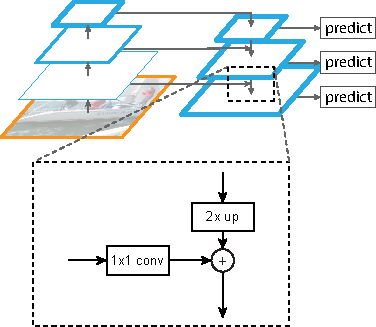
\includegraphics[]{images/fpn-lateral.pdf}
    \caption{A building block illustrating the lateral connection and
    the top-down pathway, merged by addition \cite{lin2017fpn}}
    \label{fig:fpn-lateral}
\end{figure}


\subsection{One-Stage vs Two-Stage Detectors}

Object detectors can be broadly categorized into \emph{one-stage} and \emph{two-stage} paradigms. Both ultimately predict a variable-sized set of detections $\mathcal{D} = \{(b_i, y_i, s_i)\}$, but they differ in how they structure intermediate computations and where they allocate capacity for localization vs.\ classification.

\subsubsection{Two-stage detectors.}
Two-stage methods decompose detection into proposal generation followed by proposal classification and box refinement. Let $g_{\phi}$ denote a proposal mechanism (e.g., a region proposal network operating on a shared backbone), which maps an image $x$ to a set of candidate regions $\mathcal{P}$:
$$
\mathcal{P} = g_{\phi}(x) = \{p_j\}_{j=1}^{M}.
$$
A second function $f_{\theta}$ then classifies and refines these regions to produce final detections:
$$
\mathcal{D} = f_{\theta}(x, \mathcal{P}).
$$
Operationally, the pipeline is:
\begin{enumerate}
    \item Backbone (optionally with a feature pyramid) extracts multi-scale features from $x$.
    \item A proposal generator produces a sparse set of regions $\mathcal{P}$ (typically with non-maximum suppression to reduce redundancy).
    \item Per-region features are pooled/aligned from the shared feature maps and passed to a detection head to output class scores and refined boxes.
\end{enumerate}

The idea underlying two-stage detectors is to incentivise accuracy by first generating a manageable number of promising candidates, which can then be processed and refined with more complex per-region heads. This also allows for a more efficient use of computational resources, as the second stage can focus on a smaller set of regions rather than processing the entire image densely.
But unfortunately, this approach introduces a fair amount of complexity requiring careful design.

\subsubsection{One-stage detectors.}
One-stage methods simplify the detection pipeline by predicting detections directly from the shared feature maps without an explicit proposal stage. This design is motivated by the desire to maximize throughput and reduce latency, particularly in real-time applications. This type of detection is often referred to as \emph{dense predictions} because it involves predicting detections at every spatial location of the feature maps, often having to take into account hundreds of thousands of locations per image.
Conceptually, it implements a direct mapping
$$
\mathcal{D} = h_{\psi}(x),
$$
where $h_{\psi}$ produces, for each spatial location (and possibly for multiple predefined reference shapes), joint classification scores and box parameters. The pipeline is:
\begin{enumerate}
    \item Backbone (optionally with a feature pyramid) extracts multi-scale features from $x$.
    \item Lightweight prediction heads applied densely over feature maps output $(b, y, s)$ candidates.
    \item A single-stage post-processing (e.g., top-$k$ filtering and non-maximum suppression) yields $\mathcal{D}$.
\end{enumerate}
This design maximizes throughput and simplifies the graph, but operates under severe class imbalance, due to the fact that most locations tend to be related to a generic background class, and thus the model has to learn to distinguish between a very large number of background locations and a comparatively small number of foreground locations. This imbalance is often addressed with specialized loss functions, such as the Focal Loss \cite{lin2018focalloss}, which down-weights easy-to-classify examples and focuses training on hard negatives.
The precision of the predictions often relies on effective assignment and post-processing techniques.
An alternative way of addressing this imbalance, ironically, is to use a two-stage approach, where the first stage takes care of separating the foreground (potential candidates) from the background.

\paragraph{Comparative characteristics.}
One might ask "Which paradigm is better then?" and the answer would be, as usual, "it depends". One-stage detectors are generally faster and more resource-efficient, and that is because they were intended to address the latency and throughput requirements of real-time applications. This comes at the cost of some accuracy that two-stage detectors can achieve with their more careful filtering mechanisms and (usually) more complex per-region heads that come at the cost of increased compatuational requirements and latency. And similarly one-stage detectors, they were designed to be accurate rather than fast.

Ideally one would like to have the best of both worlds, and we can find in literature a number of approaches that tries to reach two-stage performance with one-stage efficiency, such as the RetinaNet and YOLO \cite{lin2018focalloss,redmon2016yolo}.

We can summarize the main differences between one-stage and two-stage detectors as follows:
\begin{itemize}
    \item \textbf{Computation.} Two-stage: cost scales with the number of proposals $M$ (feature pooling and per-RoI head). One-stage: cost scales with the number of feature locations (and reference shapes) processed densely.
    \item \textbf{Capacity allocation.} Two-stage allocates more parameters per candidate via the second-stage head; one-stage relies on shallow, shared heads and benefits from strong multi-scale features.
    \item \textbf{Class imbalance.} One-stage training observes extreme foreground/background imbalance due to dense supervision; two-stage partially mitigates this by filtering with proposals and sampling strategies.
    \item \textbf{Latency/throughput.} One-stage typically achieves lower latency and higher FPS; two-stage often offers higher accuracy at increased computational cost.
    \item \textbf{Post-processing.} Two-stage commonly applies suppression both after proposal generation and after final classification; one-stage applies it once on dense predictions (often per class).
\end{itemize}


% \paragraph{Outlook.}
% In what follows, we instantiate these paradigms with canonical representatives: a one-stage detector with dense predictions, and a two-stage detector with proposals followed by RoI-level classification and refinement, both using feature pyramids to extract multi-scale features. We subsequently discuss anchor-based vs.\ anchor-free formulations, which apply orthogonally to both paradigms.


\subsection{Anchor-Based vs.\ Anchor-Free}

Object detectors differ not only by staging (one- vs.\ two-stage) but also by how they parameterize candidate boxes. The two prevailing choices are \emph{anchor-based} (predefined reference boxes) and \emph{anchor-free} (direct box prediction without references). This design is largely orthogonal to the staging paradigm.

\subsubsection{Anchor-based detectors}
\label{sec:anchor_based_detectors}
Let $\mathcal{A}=\{a_k\}_{k=1}^{K}$ be a set of predefined anchors tiled over feature maps. 
Each anchor $a_k=(x_a,y_a,w_a,h_a)$ serves as a reference against which a detector predicts offsets $(t_x,t_y,t_w,t_h)$ to obtain a box:
$$
x = x_a + w_a t_x \quad
y = y_a + h_a t_y \quad
w = w_a e^{t_w} \quad
h = h_a e^{t_h}
$$

Anchors are generated at multiple scales and aspect ratios per spatial location and per FPN level $\ell$ (with stride $s_\ell$), e.g.\ scales $\{s_\ell \cdot \alpha\}$ and ratios $r \in \{1\!:\!2,\,1\!:\!1,\,2\!:\!1\}$.
The number of anchors generated for each image tends to be large, but since we're considering the spatial locations of the feature maps, and not the original image, this number is still manageable, although it can still be in the order of hundreds of thousands, depending on the number of feature maps, stride, number of scales, aspect ratios and size of the image.\\

Training uses \emph{IoU-based assignment}: for ground-truth boxes $\{b_i^\ast\}$, compute $M_{ik}=\mathrm{IoU}(b_i^\ast,a_k)$; for some given $\tau_{\text{pos}}, \tau_{\text{neg}} \in [0, 1]$ mark $a_k$ positive if $M_{ik}\ge \tau_{\text{pos}}$ for some $i$, negative if $M_{ik}\le \tau_{\text{neg}}$, and ignore otherwise. 

We now have the anchors partitioned into $\mathcal{A}^+$ (positive), $\mathcal{A}^-$ (negative), and $\mathcal{A}^0$ (ignored).
Positives receive a foreground class label $y^\ast$ and regression targets $t_k$; negatives receive the background label; ignored anchors are excluded from loss computation.
Training thus optimizes
$$
\mathcal{L}
= \frac{1}{N_{\text{cls}}}\sum_{k \in \mathcal{A}^+ \cup \mathcal{A}^-} \ell_{\text{cls}}(\hat{c}_k, c_k)
\;+\;
\lambda\,\frac{1}{N_{\text{reg}}}\sum_{k \in \mathcal{A}^+} \ell_{\text{reg}}(\hat{t}_k, t_k),
$$
where $\ell_{\text{cls}}$ is the classification/objectness loss and $\ell_{\text{reg}}$ (e.g., Smooth-$L_1$ or IoU-based) is applied \emph{only} to positives.
Negatives contribute \emph{only} to classification as background; ignored anchors contribute to neither term.

\paragraph{Suppressing redundancy.}
As seen in this section, anchor-based detectors generate a large number of anchors, many of which are near-duplicates (they overlap with the same ground-truth boxes). Ideally we would like only one anchor, hence one detection, per ground-truth, therefore we need a post-processing procedure to remove these redundant detections.

This is typically done in two steps: we first keep the top-$k$ detections per level/class, where $k$ is an hyperparameter (pre-NMS step), and then we apply Non-Maximum Suppression (NMS) to remove overlaps, producing the final set $\mathcal{D}$ \cite{neubeck2006efficient}.
Given a set of competing detections $\mathcal{D} = \{(b_i, y_i, s_i)\}$, NMS iteratively selects the detection with the highest score $s_i$ and removes all other detections that overlap with it above a threshold $\tau_{\text{nms}}$ (typically $0.5$). The process continues until no detections remain above the threshold.
As a result, NMS produces a final set of detections $\mathcal{D} = \{(b_i, y_i, s_i)\}$ that are non-overlapping and have the highest scores among the competing detections.
This procedure is clearly non-differentiable, and thus it is not possible to backpropagate through it, hence we always backpropagate on the pre-NMS detections.


\subsubsection{Anchor-free detectors.}
Anchor-free methods remove the predefined anchor set $\mathcal{A}$: each feature-map location $p$ is supervised directly.
A common approach is the one used in FCOS, which assigns each location $p=(x_p, y_p)$ to at most one ground-truth box $b^\ast$ if $p \in b^\ast$ (optionally restricted to a center region and a size range matched to level $\ell$).
After assignment, the location $p$ is labeled positive with class $y^\ast$ and regression targets given by distances to the four sides of $b^\ast$:
$$
\ell_p = x_p - x^\ast_{\text{left}},\quad
t_p = y_p - y^\ast_{\text{top}},\quad
r_p = x^\ast_{\text{right}} - x_p,\quad
b_p = y^\ast_{\text{bottom}} - y_p,
$$
decoded at inference as $[x_p-\ell_p,\; y_p-t_p,\; x_p+r_p,\; y_p+b_p]$.
Locations not assigned to any box act as background in the classification loss and do not contribute to regression.
Many designs also predict a per-location quality term (e.g.\ ``centerness'') to down-weight ambiguous border locations. 
Alternative anchor-free formulations include keypoint-based representations (e.g.\ object centers or corners) with local offsets~\cite{tian2019fcos,law2019cornernet,duan2019centernet}.\\

Anchor-free models avoid anchor tuning and can better handle unusual aspect ratios, but rely on effective assignment rules (inside-box, center sampling, size ranges) and robust post-processing.

\paragraph{Comparison and practical notes.}
\begin{itemize}
    \item \textbf{Design knobs} Anchor-based: choose scales/ratios, IoU thresholds, per-level priors. Anchor-free: choose assignment region, size ranges per level, and optional quality terms.
    \item \textbf{Label assignment} Anchor-based uses $\mathrm{IoU}$ with thresholds; anchor-free uses geometric inclusion at locations (often with center sampling). Advanced heuristics (e.g., ATSS/OTA) can be applied to either family \cite{zhang2020atss,ge2021ota}.
    \item \textbf{Computational profile} Similar dense heads; anchor-free can reduce memory and labels by removing large anchor sets.
\end{itemize}



\section{RetinaNet}
% a one-stage anchor-based architecture, essentially a toned-down Faster R-CNN, this is why i'd describe it first
% Describe the its architecture and components, address that it is born to address the class imbalance problem with the Focal Loss introduction, and its intended for medical imaging applications


RetinaNet is a one-stage, anchor-based detector that combines a backbone with a feature pyramid and two lightweight, densely-applied heads (classification and regression). Its key contribution is the \emph{focal loss}, which mitigates extreme foreground/background imbalance in dense prediction~\cite{lin2018focalloss}.

\begin{figure}[h]
    \centering
    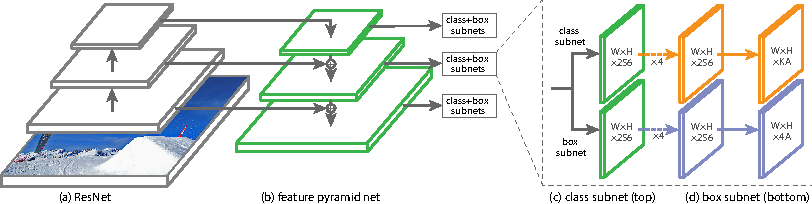
\includegraphics[page=1,width=\linewidth]{images/retinanet.pdf}
    \caption{RetinaNet architecture overview \cite{lin2018focalloss}}
    \label{fig:retinanet}
\end{figure}


\subsubsection{Architecture}
A convolutional backbone (e.g., ResNet) feeds a feature pyramid $\{P_\ell\}$ (typically $P_3$--$P_7$). 
At each pyramid level $\ell$ with spatial size $H_\ell \times W_\ell$, and stride $s_\ell$, a set of $A$ anchors per location is tiled. 
Two subnetworks are applied at each level of the pyramid, producing per-anchor outputs:
\begin{itemize}
    \item \emph{Classification head:} a small CNN produces per-class logits $\hat{z}_{\ell,ij,a,c}$, using independent sigmoids (no softmax) over $c \in \{1,\dots,K\}$.
    \item \emph{Regression head:} a parallel CNN predicts box deltas $\hat{t}_{\ell,ij,a}=(\hat{t}_x,\hat{t}_y,\hat{t}_w,\hat{t}_h)$.
\end{itemize}

Once we obtain the structured outputs from the network, we apply the post-processing steps discussed 
in Section~\ref{sec:anchor_based_detectors} to discard redundant detections.

\paragraph{Focal Loss.}

As previously mentioned, RetinaNet introduced the \emph{focal loss} to address the extreme class imbalance in dense predictions.
It essentially down-weights easy to classify examples and focuses training on hard negatives (Figure~\ref{fig:focal-loss}), which is particularly useful in medical imaging where the background class can dominate the training set. To do so it adds a modulating factor $(1-p_t)^\gamma$ to the cross-entropy loss, with a focus parameter $\gamma$. The focal loss is hence defined as follows:

$$
\mathrm{FL}(p_t) = -\,\alpha\,(1-p_t)^{\gamma}\,\log(p_t),
$$
with typical $\alpha{=}0.25$, $\gamma{=}2$.\\
\begin{figure}[h]
    \centering
    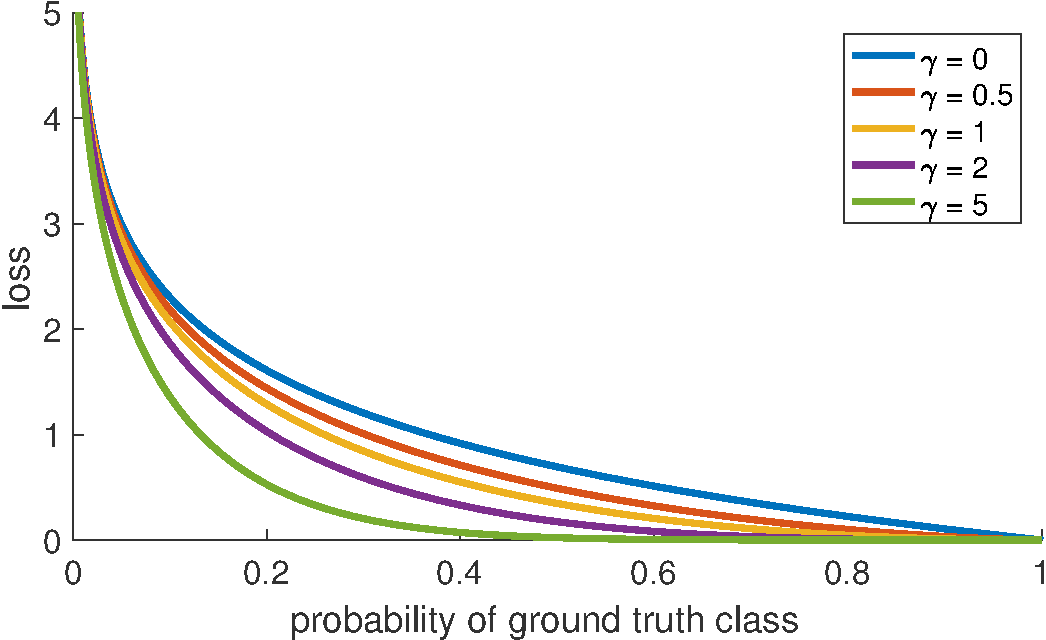
\includegraphics[width=0.55\linewidth]{images/focal-loss.pdf}
    \caption{Focal loss at different $\gamma$ values \cite{lin2018focalloss}. When $\gamma=0$, it is equivalent to cross-entropy loss. As $\gamma$ increases, the loss focuses more on hard examples, down-weighting easy ones.}
    \label{fig:focal-loss}
\end{figure}


\section{Faster R-CNN}
% two-stage anchor-based architecture, the most common one and the one that is used in most of the literature.
% Describe its components, RPN, RoI pooling etc., it is the culmination of the R-CNN family of architecutres.
% f

Faster R-CNN is a two-stage, anchor-based detector that couples a Region Proposal Network (RPN) with a per-region classifier and regressor~\cite{ren2016fasterrcnn}. A shared backbone (we consider one using FPN) feeds both stages.

\begin{figure}[h]
    \centering
    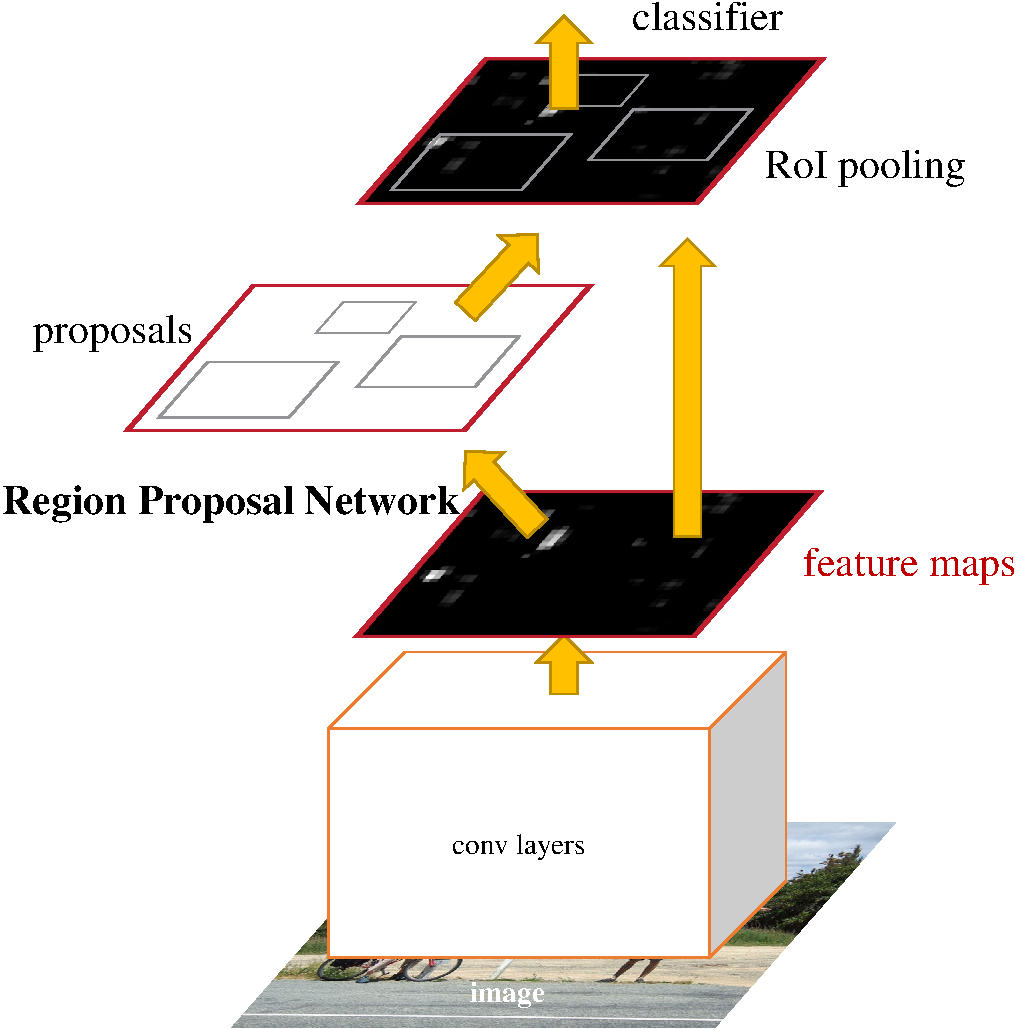
\includegraphics[width=0.6\linewidth]{images/fasterrcnn.pdf}
    \caption{Faster RCNN architecture overview \cite{ren2016fasterrcnn}}
    \label{fig:fasterrcnn}
\end{figure}


\subsubsection{Region Proposal Network (RPN).}
At each feature-map location and for $A$ anchors $a_k=(x_a,y_a,w_a,h_a)$, the RPN predicts:
\begin{itemize}
    \item objectness logits $\hat{o}_k$ (binary);
    \item box deltas $\hat{t}_k=(\hat{t}_x,\hat{t}_y,\hat{t}_w,\hat{t}_h)$.
\end{itemize}
At this stage we do not have any class information, but rather we unify all classes into a single \emph{object} against a \emph{background} class, hence the binary classification. We call \emph{objectness} the probability that an anchor contains an object, regardless of its initial class. Such probability is typically obtained by applying a sigmoid activation to the logits $\hat{o}_k$.\\
Anchors are assigned to ground-truth boxes by IoU thresholds: positives $\mathcal{A}^+$, negatives $\mathcal{A}^-$, ignored $\mathcal{A}^0$. Positives receive class $1$ and regression targets $t_k$ (standard parameterization),
$$
t_x=\frac{x^\ast-x_a}{w_a},\quad
t_y=\frac{y^\ast-y_a}{h_a},\quad
t_w=\log\frac{w^\ast}{w_a},\quad
t_h=\log\frac{h^\ast}{h_a}.
$$

At the end of the RPN, we filter the proposals by objectness score $\hat{o}_k$ and apply non-maximum suppression (NMS) to obtain a sparse set of proposals $\mathcal{P}$, which are then passed to the second stage.\\

We notice how the RPN is a fully convolutional network, therefore the size of input has not to be fixed, although it will increase the number of anchors and thus the computational cost.

\paragraph{Second-stage head.}
The second stage process starts with RoIAlign, a procedure that pools features from the shared backbone for each proposal into a fixed-size tensor $F_j$ (e.g., $7{\times}7{\times}C$) without quantization errors \cite{he2018maskrcnn}. This is done by bilinear interpolation of the feature maps at the proposal locations, which avoids the quantization issues that arise with max pooling, that was a common issue in the original R-CNN architectures using RoIPooling instead.

A per-RoI head predicts:
\begin{itemize}
    \item class logits $\hat{z}_{j,c}$ for $c\in\{1,\dots,K\}$ (softmax over $K{+}1$ including background);
    \item refined box deltas $\hat{u}_{j,c}$ (class-specific) or $\hat{u}_j$ (class-agnostic).
\end{itemize}
With labels $(y_j^\ast, u_j^\ast)$ from matching $p_j$ to ground truth, the loss is
$$
\mathcal{L}_{\text{RoI}}
=\frac{1}{N_{\text{roi}}}\sum_{j}\ell_{\text{ce}}(\hat{z}_{j},y_j^\ast)
+\lambda_{\text{roi}}\frac{1}{N_{\text{pos}}}\sum_{j\in\mathcal{P}^+}\ell_{\text{reg}}(\hat{u}_{j,(y_j^\ast)},u_j^\ast),
$$
where regression applies only to positives $\mathcal{P}^+$.\\

Training of Faster R-CNN is performed end-to-end, with both the RPN and the second-stage detection head sharing the same backbone features. To keep the optimization stable, a sampling strategy is used at both stages to balance the large number of negative examples against the relatively few positives: mini-batches are constructed with a fixed foreground-background ratio for anchors in the RPN and for RoIs in the second stage. The assignment of positives and negatives relies on IoU thresholds -- for the RPN, anchors above a high threshold are treated as positives and those below a low threshold as negatives, while intermediate cases may be ignored; for the RoI head, proposals with sufficiently high IoU to a ground-truth box are considered foreground, and the rest background. During backpropagation, gradients propagate through the RoIAlign operation and further into the shared backbone, but not through the non-differentiable proposal selection and NMS steps, which are treated as fixed post-processing operations. Instead we backpropagate through the pre-NMS detections, with analogous loss functions as the ones used in the RoI heads that uses the notion of objectness and anchor's coordinates, allowing the model to learn to produce better proposals and detections.


% \subsection{DETR}
% a one-stage anchor-free architecture, the first to introduce the transformer architecture in object detection, it is a fully end-to-end architecture that does not rely on anchors or region proposals, but rather directly predicts the bounding boxes and class labels in a single pass. Unfortunately, it is not suitable for our use case due to its large needs of data.

\section{Evaluation Metrics: Average Precision and Average Recall}
Explain the need to formally define evaluation metrics as COCO's definitions are shaky, seems like everyone's using them but no one ever explains them.

\section{Explainability in Deep Learning}
Quick introduction of explainability in deep learning, highlighting how models are essentially black boxes and the need to understand, although partially, their inner workings. This need is even more pronounced in the medical field, where explainability is a requirement for clinical acceptance and regulatory compliance. Highlight how explainability methods, especially the ones that we are going to cover, are desinged to provide \emph{insights} into the model's decision-making process, it does not make it fully explainable, but rather makes it a gray-box model, which is still better than a black box.
Trainsition to CAMs for computer vision tasks

\subsection{Class Activation Maps (CAM)}
What are CAMs, how they work, and their (usual) limitations. Describe GradCAM as a gradient-based method and then explain why it is problematic for object detection tasks due to their sensitivity to the structured outputs and the non-differentiable post-processing steps. 

\subsection{Adaptations for Object Detection}
Discuss gradient-free CAM methods ScoreCAM, SS-CAM and EigenCAM, highlighting how they can be adapted to work with object detection outputs. there's a bit of math involved here as we got to pinpoint what fails in their original implementations and how we can fix it.

\chapter{Data and Preprocessing}
\label{chap:data-and-preprocessing}
\section{Datasets: NLST and DLCSD24}
The development and evaluation of computer-aided detection systems for pulmonary nodules heavily rely on comprehensive and diverse datasets. In this work, we leverage two distinct datasets: the National Lung Screening Trial (NLST) \cite{nlst_data} and the Duke Lung Cancer Screening Dataset 2024 (DLCSD24) \cite{dlcsd24}. Each dataset presents unique multiple slices/volumes of CT scans, annotated with pulmonary nodule locations, necessary for training and validating our detection models.

Both datasets will serve as 2D datasets, meaning that each slice of the CT scan will be treated as a separate image. The slicing will be done on axial planes of the patient, which is the most common orientation for viewing CT scans.
The NLST dataset already comes as a collection of 2D slices on the axial plane, while the DLCSD24 dataset comes as a collection of 3D volumes that will have to be sliced, and possibly only a subset of slices of interest -- namely those containing nodules -- will be retained for training and evaluation.

\subsection{National Lung Screening Trial (NLST)}
The NLST is a large-scale, randomized controlled trial conducted by the National Cancer Institute (NCI) to determine if spiral computed tomography (CT) screening could reduce lung cancer mortality compared to standard chest X-ray. It enrolled over 53,000 participants at 33 sites across the United States. For the purpose of this study, the NLST dataset provides a vast collection of low-dose CT scans, which are invaluable for training nodule detection models.
Unfortunately, only a small subset of the NLST dataset includes annotations for pulmonary nodules, and these only cover malignant nodules.
After this filtering, we are left with approximately 9000 scans, each containing on average one nodule, for a total of around 9000 nodules of size greater or equal to 4 mm.
Regardless the absence of benign annotations, the NLST can be effectively utilized to teach a model to recognize nodule-like structures. Furthermore, the NLST dataset can serve as an excellent source for pre-training detection models, allowing them to learn general features of pulmonary nodules before fine-tuning on datasets with more detailed annotations.


\subsection{Duke Lung Cancer Screening Dataset 2024 (DLCSD24)}
The Duke Lung Cancer Screening Dataset (DLCSD24) is a large-scale, annotated collection of low-dose thoracic CT scans designed to support research in lung nodule detection and cancer risk assessment using modern CT technology \cite{dlcsd24}. The dataset was compiled from screening examinations conducted at the Duke University Health System between January 2015 and June 2021, and consists of 1,613 CT volumes drawn from a pool of 2,061 patients, with additional cases reserved for future releases. Within these scans, a total of 2,487 nodules were annotated through a semi-automated pipeline in which a detection model, pre-trained on the LUNA16 dataset, generated candidate nodules that were subsequently verified and refined using radiology reports and expert review. Manual adjustments were performed by a medical student and a fellowship-trained cardiothoracic radiologist, and independent spot checks confirmed that the resulting annotations achieved an accuracy exceeding ninety percent. The dataset is released in multiple parts, with versioned updates hosted on Zenodo to ensure accessibility and reproducibility, and represents the first publicly available, large-scale screening dataset acquired with up-to-date CT protocols. As such, DLCSD24 provides a valuable benchmark for developing and evaluating artificial intelligence models for lung nodule detection and classification in contemporary clinical practice.
Compared to the NLST, the DLCSD24 dataset offers both malignant and benign nodule annotations, despite with a severe imbalance with a ratio of approximately 1:10. The nodules in this dataset are also generally smaller, a property that makes them more challenging to detect. The DLCSD24 dataset is therefore particularly well-suited for training and evaluating nodule detection models, as it provides a more comprehensive representation of the types of nodules that may be encountered in clinical practice.

\subsubsection{Slice Extraction from 3D Volumes}
The DLCSD24 dataset is provided as a collection of 3D CT volumes. As previously stated in this chapter, we want to extract a 2D dataset from these volumes by slicing them along the axial plane. This is done by iterating through each volume, and extracting each slice as a separate image. If we were to extract all slices, we would end up with an extremely large dataset, with the majority of the data being non-informative, as most slices do not contain any nodules. To mitigate this, we use the provided annotations to identify slices that contain nodules, and only retain those slices for our 2D dataset. This results in a more manageable dataset size, while still retaining the most relevant information for nodule detection. 

\begin{figure}[h]
    \centering
    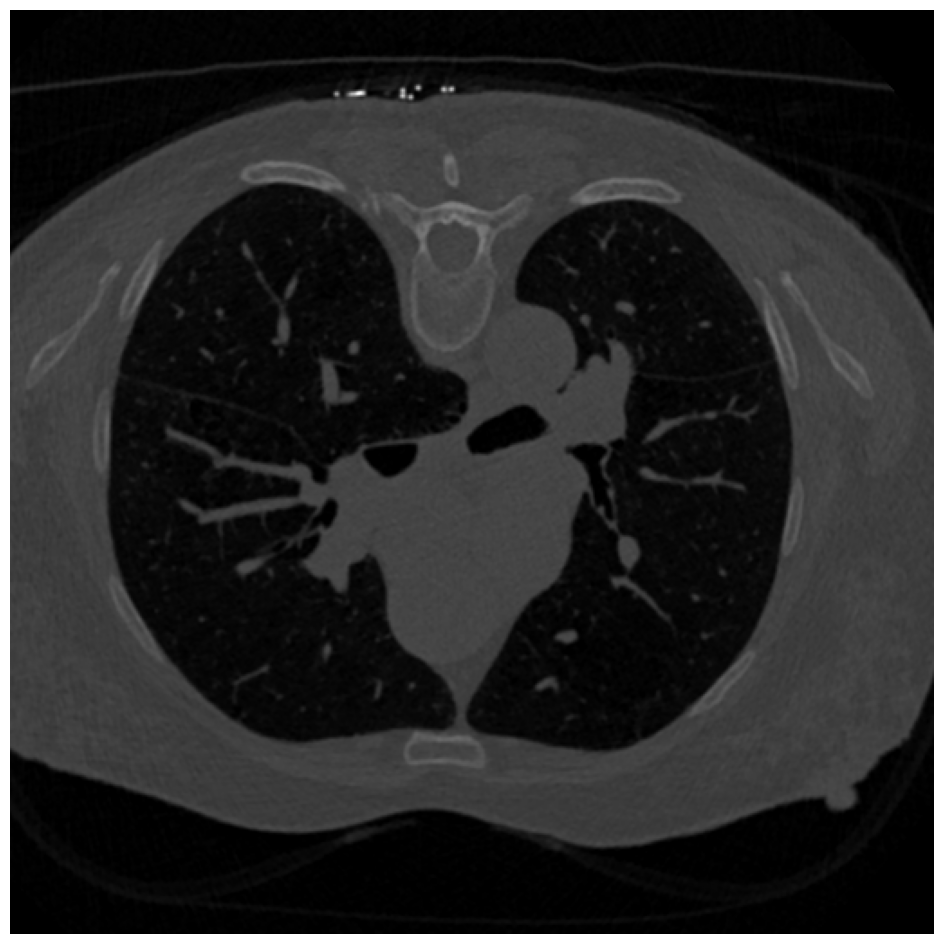
\includegraphics[width=0.6\linewidth]{images/dlcs_sample_unprocessed.png}
    \caption{Example of an unprocessed slice extracted from the DLCSD24 dataset.}
    \label{fig:dlcs-sample-unprocessed}
\end{figure}

% The size of the resulting 2D dataset depends on the thickness of the slices in the original 3D volumes, but in order to have a consistent size across all scans, we resample all volumes to have a slice thickness of 1.25mm, height and width spacing of 0.7mm, and then extract all slices containing nodules, along with a few slices before and after each nodule-containing slice to provide some context. This results in a final dataset of approximately 10,000 slices, each containing at least one nodule.

% This resampling step is crucial, as it ensures that all slices have the same resolution and spacing, which allows models to have a consistent spatial understanding of the images. 


\section{Preprocessing Pipeline}
\label{sec:preprocessing}
% Resampling, and HU clipping, explaining why we're clipping and why those ranges and not others, this is supported by the HU table.
% We might include here also discarded preprocessing steps, such as outlier removal (although it was a post-process step), and lung masking through morphological operations.

The preprocessing pipeline is a crucial step in preparing the CT scan data for effective analysis and model training. This pipeline involves several steps, including resampling, normalization, and Hounsfield Unit (HU) clipping, each of which plays an significant role in enhancing the quality and consistency of the input data and therefore quality of the detection.

\subsubsection{Resampling}
\label{sec:resampling}
CT scans can vary significantly in terms of their spatial resolution and slice thickness (a voxel might represent a differently sized parallelepiped in millimeters depending on the scan configurations), which can introduce inconsistencies when training machine learning models. To address this, we resample all CT scans to a uniform voxel (pixels for the NLST dataset) size of 1.25mm in the axial direction and 0.7mm in the coronal and sagittal directions.
These sizes were chosen according to \cite{tushar2025ailunghealthbenchmarking} as they represent a good compromise between preserving anatomical detail and managing computational resources.
This resampling is performed using bilinear interpolation, which helps to maintain the integrity of the anatomical structures while ensuring that all scans have a consistent spatial resolution.
For the DLCSD24 dataset, this resampling is performed before the slice extraction step on the entire 3D volume. Such operation is performed usign the MONAI framework \cite{monai}.

As for the NLST dataset, since it is already provided as a collection of 2D slices, we only need to ensure that each slice has the correct in-plane resolution of 0.7mm. If any slice does not meet this requirement, it is resampled using bilinear interpolation to achieve the desired resolution and it has been performed using the SimpleITK library \cite{lowekamp2013simpleitk} to extract the slices metadata and resample using its built-in resampler. The output size, given the desired spacing, original size and current spacing, is computed as follows:
$$
\text{output\_size} = \left( \left\lfloor\frac{S_1 \cdot \delta_1}{\delta_1^\prime}\right\rceil, \left\lfloor\frac{S_2 \cdot \delta_2}{\delta_2^\prime}\right\rceil, 1 \right)
$$

Where \(S_i\) is the original size along dimension \(i\), \(\delta_i\) is the original spacing along dimension \(i\), and \(\delta_i^\prime\) is the desired spacing along dimension \(i\). The output size is rounded to the nearest integer to ensure that it represents a valid number of pixels. Since the NLST dataset is already 2D, the output size for the third dimension is set to 1 as a dummy value.

\paragraph{Ablation Study Design:}
To empirically validate the effectiveness of the resampling step, an ablation study was designed. The performance of the Faster R-CNN model will be compared across two experimental conditions: 
\begin{itemize}
    \item \textbf{Baseline:} The model trained on the original dataset without any resampling.
    \item \textbf{Resampled:} The model trained on the dataset after applying the resampling step.
\end{itemize}
For this experiments we used the EfficientNetV2-S backbone \cite{tan2020efficientnet} and the results of this ablation study are presented in Figure \ref{fig:resampling-ablation}.
\begin{figure}[h]
    \centering
    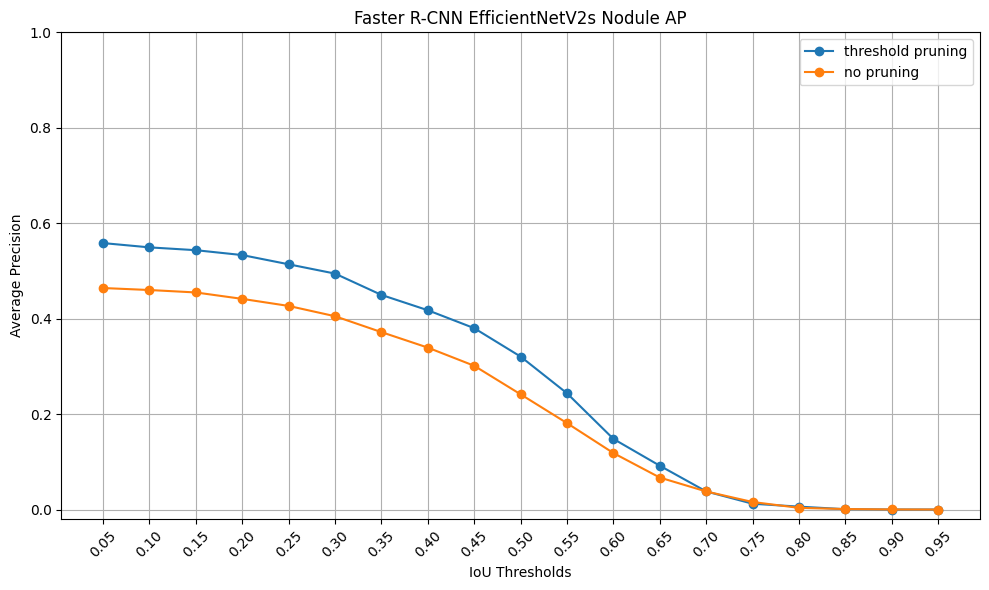
\includegraphics[width=0.8\linewidth]{images/resampling-ablation.png}
    \caption{Average Precision at varying IoU thresholds for the resampling ablation study.}
    \label{fig:resampling-ablation}
\end{figure}
As we can see from the results, the resampling step has a significant positive impact on the model's performance, particularly at higher IoU thresholds. This demonstrates the importance of having a consistent spatial resolution across all scans, validating the effectiveness of the resampling step in the preprocessing pipeline.

\subsubsection{Hounsfield Unit Clipping}
\label{sec:hu-clipping}
Hounsfield Units (HU) are a quantitative scale for describing radiodensity in medical CT imaging. Different tissues and materials in the body have characteristic HU values, which can be used to differentiate between them. Table~\ref{tab:hu-scale} summarizes the typical HU ranges for various substances commonly found in CT scans. For our purposes, we focus on the range from -1000 HU (representing air) up to +500 HU to include soft and hard tissues, while escluding extremely high values that could correspond to implants or artifacts.
\begin{table}[h!]
    \centering
    \begin{tabular}{|l|c|}
    \hline
    \textbf{Substance} & \textbf{HU Range} \\ \hline
    Air & $-1000$ \\ \hline
    Lung & $-700 \ \text{to} \ -600$ \\ \hline
    Fat & $-120 \ \text{to} \ -50$ \\ \hline
    Water & $0$ \\ \hline
    Cerebrospinal fluid & $+15$ \\ \hline
    Renal Parenchyma & $+30$ \\ \hline
    Blood & $+13 \ \text{to} \ +75$ \\ \hline
    Muscle & $+35 \ \text{to} \ +55$ \\ \hline
    Liver & $+40 \ \text{to} \ +60$ \\ \hline
    Soft tissue, IV Contrast & $+100 \ \text{to} \ +300$ \\ \hline
    Bone (Cancellous) & $+300 \ \text{to} \ +400$ \\ \hline
    Bone (Cortical) & $+500 \ \text{to} \ +1900$ \\ \hline
    Metal & $>+3000$ \\ \hline
    \end{tabular}
    \caption{Hounsfield Unit (HU) ranges of different substances.}
    \label{tab:hu-scale}
\end{table}


\subsubsection{Slice Selection Algorithms}
\label{sec:dataset_pruning}
% Explain the need for slice selection algorithms in this 2D setting, as some might not contain relevan information (nodule mass). explain the statistical approach, the sliding window approach and finally the simple thresholding approach.
A preliminary analysis revealed that the model's performance on the Duke Lung Cancer Screening (DLCS) dataset was significantly lower than on the National Lung Screening Trial (NLST) dataset. This discrepancy is attributed not only to the model's limitations but also to the inherent challenges of the DLCSD24 data itself, primarily the smaller and more variable size of nodules and the nature of the volumetric annotations.

After a brief analysis became apparent that a significant portion of the extracted 2D slices did not contain any nodules or relevant anatomical structures. This is particularly true for the upper and lower regions of the extracted nodules, where the section of the cancerous tissue is minimal or non-existent (see Figure~\ref{fig:non-visible-nodule}).

\begin{figure}[h]
    \centering
    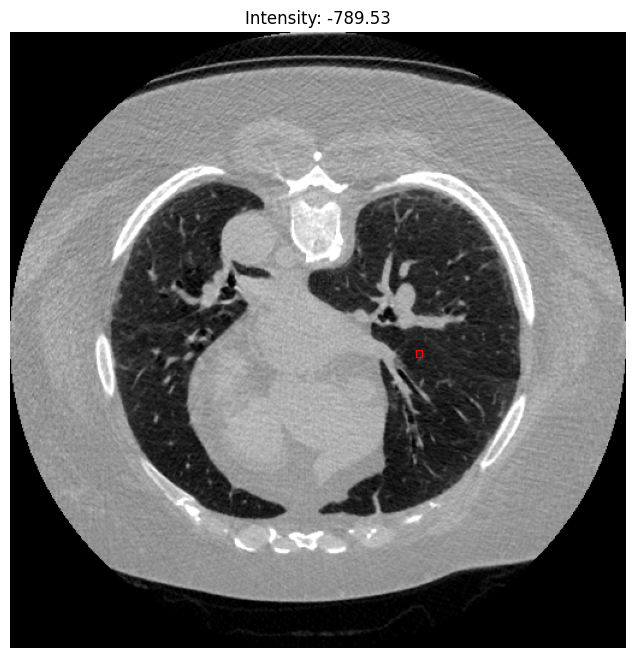
\includegraphics[width=0.6\linewidth]{images/non-visible-nodule-1.png}
    \caption{Example of a slice with an annotated nodule (at the indicated depth) that does not contain any visible tissue from the nodule itself. At the top the mean intensity expressed in Hounsfield Units (HU) of the area within the annotation. }
    \label{fig:non-visible-nodule}
\end{figure}

The strategy of extracting every 2D slice from a 3D volumetric bounding box is susceptible to annotation inaccuracies. Volumetric annotations are rarely perfect, often including slices at the superior and inferior extremes where the nodule is barely visible or entirely absent. Training the model on these ``empty" or noisy slices can introduce a significant amount of label noise, potentially degrading its performance by forcing it to learn from irrelevant or misleading examples.

To mitigate this, a dataset pruning strategy was developed to selectively remove these low-information slices. Several approaches were investigated to identify and remove them in a principled manner.

\subsubsection{Exploration of Pruning Strategies}
The core assumption behind our pruning is that slices containing predominantly healthy lung tissue or air will have a significantly lower average Hounsfield Unit (HU) intensity within the annotated bounding box compared to slices containing dense tumorous tissue. Based on this, the following strategies were explored:

\paragraph{Statistical Outlier Detection:} This initial approach, detailed in Algorithm \ref{alg:stat-pruning}, involved calculating the median ($\tilde{m}$) and Interquartile Range (IQR) of the mean bounding box intensities for all slices belonging to a single nodule. Slices with intensities considered to be low-end outliers were removed. However, this method proved to be overly aggressive, eliminating a substantial number of slices ($\sim$50\% of the dataset), including many that contained valuable information.

\begin{algorithm}[H]
    \caption{Strategy 1: Statistical Pruning}
    \label{alg:stat-pruning}
    \DontPrintSemicolon
    \SetAlgoLined
    \setstretch{1.2}

    \SetKwInOut{Input}{Input}
    \Input{
        SlicesForNodule: a list of (slice, mean\_intensity) pairs for one nodule\;
        $\alpha$: an adjustment factor (e.g., 1.5)
    }
    \SetKwData{keptSlices}{kept\_slices}
    \SetKwData{meanIntensities}{mean\_intensities}
    
    \BlankLine
    
    $\meanIntensities \gets$ [s.mean\_intensity for s in SlicesForNodule]\;
    Q1 $\gets$ FirstQuartile($\meanIntensities$)\;
    IQR $\gets$ InterquartileRange($\meanIntensities$)\;
    threshold $\gets$ Q1 - ($\alpha \times$ IQR)\;
    
    \BlankLine
    $\keptSlices \gets \{\}$\;
    \ForAll(){(slice, intensity) \textup{in} SlicesForNodule}{
        \If{intensity $\geq$ threshold}{
            $\keptSlices$.add(slice)\;
        }
    }
    \Return{$\keptSlices$}\;
\end{algorithm}


This approach, although being statistically sound, it tries to estimate properties of the mean intensity distribution, namely median and IQR, of each sample given a very limited number of slices for each nodule. This limitation often leads to an overly aggressive pruning, as the statistical estimates may not accurately reflect the true distribution of intensities.
It may also happen that if a given annotation is particularly noisy, shallow or generally mostly uninformative, the statistical properties of the mean intensity distribution may be skewed, leading to the opposite effect, removing informative slices as they might be detected as outliers of the distribution.

\paragraph{Sliding Window Approach:} To incorporate spatial locality, a sliding window of size $K$ was moved along the z-axis of each nodule (slices sorted by height). The window position that maximized the cumulative mean intensity was considered to contain the core of the nodule, as shown in Algorithm \ref{alg:sliding-window-pruning}. While this produced more coherent results, it was sensitive to the choice of $K$ and the full strategy (testing all possible values of $K$ and using an elbow method to choose the best one) proved overly complex.

\begin{algorithm}[H]
    \caption{Strategy 2: Sliding Window Pruning (fixed K)}
    \label{alg:sliding-window-pruning}
    \DontPrintSemicolon
    \SetAlgoLined
    \setstretch{1.2}
    
    \SetKwInOut{Input}{Input}
    \Input{
        SortedSlices: a list of slices for one nodule, sorted by z-index\;
        K: the size of the sliding window
    }
    \SetKwData{intensities}{intensities}
    \SetKwData{maxSum}{max\_sum}
    \SetKwData{bestStart}{best\_start\_index}

    \BlankLine
    
    $\intensities \gets$ [s.mean\_intensity for s in SortedSlices]\;
    $\maxSum \gets -\infty$\;
    $\bestStart \gets -1$\;
    
    \For{$i \gets 0$ \textup{to} len(SortedSlices) - K}{
        current\_sum $\gets$ Sum of $\intensities$ from index $i$ to $i+K-1$\;
        \If{current\_sum $>$ $\maxSum$}{
            $\maxSum \gets$ current\_sum\;
            $\bestStart \gets i$\;
        }
    }
    \Return{sub-list of SortedSlices from $\bestStart$ to $\bestStart+K-1$}\;
\end{algorithm}

Similarly to the statistical approach, this method ended up being overly aggressive, eliminating almost $40\%$ of the original data. This behaviour is due to the very shallow curve generated by the best cumulative mean intensity for each $K$. Meaning that the elbow point, supposed to indicate the optimal $K$ was often not well-defined. As a result, even when the annotation where well positioned, the method would still exclude some slices, although informative.
Nonetheless, the resulting dataset was definitely more coherent compared to the statistical approach.

\paragraph{Informed HU Thresholding:} The final and most effective strategy was a simple yet informed threshold, described in Algorithm \ref{alg:threshold-pruning}. Based on the typical HU values for soft tissue, a threshold of -750 HU was established. Any slice where the average intensity within the ground truth bounding box fell below this value was removed. This method is less aggressive and more clinically grounded, resulting in the exclusion of approximately 12.5\% of the total slices.

\begin{algorithm}[H]
    \caption{Strategy 3: Informed HU Thresholding}
    \label{alg:threshold-pruning}
    \DontPrintSemicolon
    \SetAlgoLined
    \setstretch{1.2}

    \SetKwInOut{Input}{Input}
    \Input{
        SlicesForNodule: a list of (slice, mean\_intensity) pairs for one nodule\;
        $T_{HU}$: the HU threshold (-750 HU)
    }
    \SetKwData{keptSlices}{kept\_slices}
    
    \BlankLine
    
    $\keptSlices \gets \{\}$\;
    \ForAll(){(slice, intensity) \textup{in} SlicesForNodule}{
        \If{intensity $\geq T_{HU}$}{
            $\keptSlices$.add(slice)\;
        }
    }
    \Return{$\keptSlices$}\;
\end{algorithm}

Despite its simplicity, this approach effectively balances the need to remove uninformative slices while preserving potentially informative ones.
Differently from the other methods, it does not need to estimate properties from the data distribution of a single nodule, but rather relies on established clinical knowledge about HU values, making it more robust to annotation noise and variability in nodule appearance.

\paragraph{Ablation Study Design}
To empirically validate the effectiveness of the final Informed HU Thresholding strategy, an ablation study was designed. The performance of the Faster R-CNN model will be compared across two experimental conditions:
\begin{itemize}
    \item \textbf{Baseline:} The model trained on the full dataset of all extracted slices.
    \item \textbf{Pruned:} The model trained on the dataset after applying the pruning strategy from Algorithm \ref{alg:threshold-pruning}.
\end{itemize}
This experiment was conducted using the EfficientNetV2-S backbone and the results of this ablation study are presented in Figure \ref{fig:threshold-pruning-ablation}.

\begin{figure}[h]
    \centering
    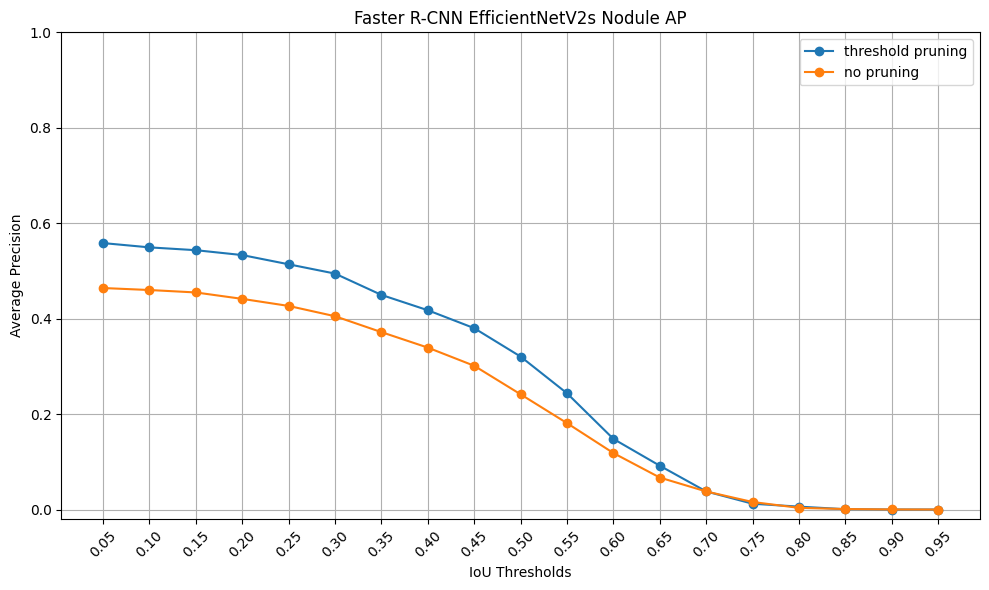
\includegraphics[width=0.8\linewidth]{images/threshold-pruning-ablation.png}
    \caption{Average Precision at varying IoU thresholds for threshold pruning ablation study.}
    \label{fig:threshold-pruning-ablation}
\end{figure}

The results clearly demonstrate the positive impact of the pruning strategy on the model's performance, particularly at higher IoU thresholds. This indicates that removing uninformative slices helps the model to focus on learning from relevant examples, thereby improving its detection capabilities. The Informed HU Thresholding strategy effectively enhances the quality of the training data, validating its inclusion in the preprocessing pipeline.\\

In addition to this ablation study, we also conducted a negative control experiment by training the same model on the dataset using the excluded slices only amounting to approximately 12.5\% of the original data ($\sim$1000 slices). The results of this experiment -- despite the limited amount of data -- showed an extremely poor performance, with an AP@5:95 of only 0.01, confirming that the excluded slices were indeed largely uninformative for the task of nodule detection.



\subsubsection{Three-channel Input Representation}
\label{sec:2.5d_approach}

While a 2D slice-based approach offers significant computational advantages over a full 3D analysis, it inherently discards the volumetric context that is crucial for accurate nodule characterization. In a single 2D slice, a small pulmonary nodule can be morphologically indistinguishable from a cross-section of a blood vessel or other anatomical structures. Radiologists naturally scroll through adjacent slices to observe how a feature evolves in the third dimension (the z-axis) to make a confident diagnosis.

To address this limitation without incurring the prohibitive memory and computational costs of full 3D convolutional networks, we adopt a multi-channel input representation, often referred to as a \textbf{2.5D approach}. This method synthesizes local volumetric information into a format that is directly compatible with standard 2D CNN architectures.
The idea comes from the observation that the pretrain used from ImageNet1K is on RGB images \cite{russakovsky2015imagenet}, which have already have three channels, while CT scans are single channel grayscale images, so we can leverage this by stacking adjacent slices to create a three-channel input, rather than copying the same slice three times.

For a given target slice at position $z$, which contains a nodule annotation, we construct a three-channel input tensor analogous to a standard RGB image. Instead of Red, Green, and Blue channels, the three channels are populated with grayscale intensity information from adjacent CT slices:

\begin{itemize}
    \item \textbf{Channel 1:} The preceding slice in the sequence, at position ($z-1$).
    \item \textbf{Channel 2:} The current target slice, at position ($z$).
    \item \textbf{Channel 3:} The subsequent slice in the sequence, at position ($z+1$).
\end{itemize}
If there is no available preceding or subsequent slice (e.g., at the beginning or end of a scan), the missing channel is filled by duplicating the target slice.
This technique offers several key advantages for our methodology:

\begin{itemize}
    \item \textbf{Enhanced Feature Representation:} It provides the model with crucial, localized 3D context. By seeing the preceding and subsequent slices, the network can learn to discern the characteristic spherical shape of a nodule as it changes across slices, helping to differentiate it from elongated, tubular structures like blood vessels.

    \item \textbf{Compatibility with Pre-trained Models:} It aligns perfectly with the three-channel input structure of the canonical backbone architectures used in this work (ResNet50, MobileNetV2, and EfficientNetV2-S). This allows for the direct and effective use of weights pre-trained on ImageNet1K \cite{russakovsky2015imagenet}, a dataset of three-channel RGB images, which is a cornerstone of modern transfer learning.

    \item \textbf{Computational Efficiency:} The approach processes three 2D slices at a time using standard 2D convolutions, thereby retaining the computational efficiency of a 2D pipeline. This avoids the exponential increase in parameters and memory usage associated with 3D convolutional layers, making the method accessible on commercial GPU hardware.
\end{itemize}

In cases where a preceding or subsequent slice is not available (i.e., for the very first or last slice in a nodule's sequence), the missing channel is populated by duplicating the target slice $z$. This padding technique ensures a consistent input dimension for all samples fed to the network.

\paragraph{Ablation Study Design:}
To empirically validate the effectiveness of the 2.5D approach, an ablation study was designed. The performance of the Faster R-CNN model will be compared across two experimental conditions:
\begin{itemize}
    \item \textbf{Single-channel Input:} The model trained using only the target slice as a single-channel grayscale image, with the channel duplicated to create a three-channel input.
    \item \textbf{Three-channel Input:} The model trained using the 2.5D approach, with the target slice and its adjacent slices forming a three-channel input. 
\end{itemize}
To conduct this study we used the Faster R-CNN model with an EfficientNetV2-S backbone on the DLCSD24 dataset and the results are presented in Figure \ref{fig:3channel-ablation}.

\begin{figure}[h]
    \centering
    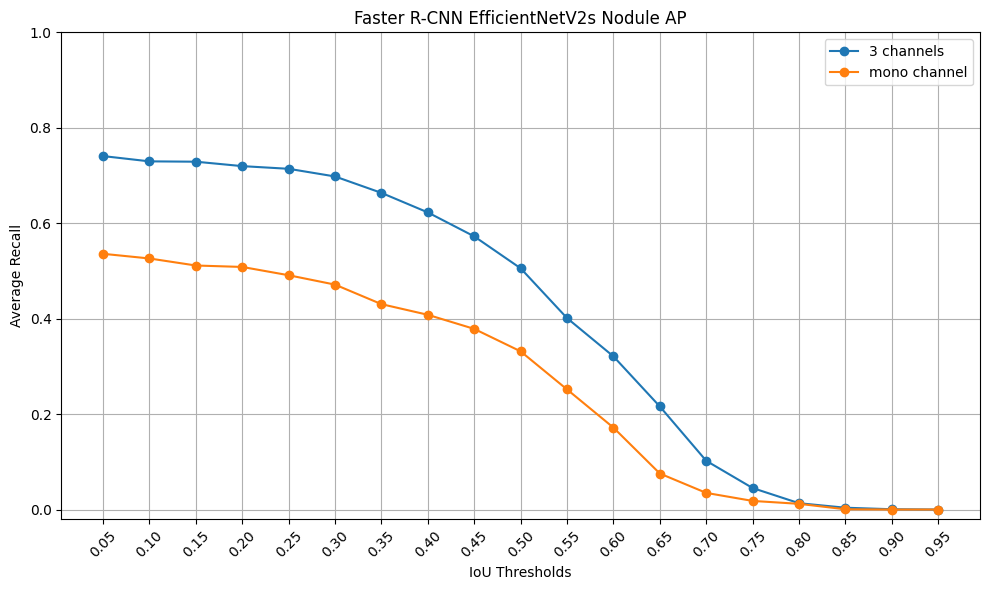
\includegraphics[width=.8\linewidth]{images/3-channel-ablation.png}
    \caption{Average Precision at varying IoU thresholds for 3-channel ablation study.}
    \label{fig:3channel-ablation}
\end{figure}

We can clearly see the impact that the 2.5D approach has on the model's performance, with a significant increase in Average Precision across all IoU thresholds when using the three-channel input representation. This demonstrates the value of incorporating local volumetric context into a 2D detection framework, validating the effectiveness of the 2.5D approach for pulmonary nodule detection. Given these results, the 2.5D three-channel input representation is adopted as the standard input format for all subsequent experiments in this thesis.

\section{Classification Dataset}
For the classification task, we derive a dataset from the DLCSD24 dataset, the only one of the two that contains both benign and malignant nodule annotations.
Each patch is labeled according to the malignancy of the nodule it contains, resulting in a binary classification problem (benign vs malignant).
The dataset is constructed by extracting patches around each annotated nodule, ensuring that the nodule is centered within the patch. Before any extraction takes place, each CT-Scan undergoes the same preprocessing pipeline described in Section \ref{sec:preprocessing}, including resampling to a uniform voxel size and HU clipping.
The classes of this dataset are highly imbalanced, with a ratio of approximately 1:10 between benign and malignant nodules. To address this imbalance during training, we employ an oversampling strategy, where benign nodules are cloned a number of times in the dataset to match the number of malignant nodules. This approach help to ensure that the model is exposed to a balanced representation of both classes during training, which is crucial to prevent bias towards the majority class and to improve the model's ability to generalize to unseen data.

\subsection{Additional Preprocessing for Classification}
In addition to the preprocessing steps outlined in Section~\ref{sec:preprocessing}, the classification dataset requires further preprocessing to ensure that the input patches are of a consistent size and format suitable for training a classification model.

\subsubsection{Panning and Resizing}
The classification dataset is constructed by extracting zoomed-out patches centered around each annotated nodule. The reason behind this choice is to provide the classification model with sufficient contextual information about the nodule's surroundings, and to ensure that the nodule is fully contained within the patch, accounting for potential annotation's inaccuracies. The size of these patches is determined based on the specific nodule size, ensuring that smaller nodules are not lost in overly large patches, while larger nodules are fully captured.
To achieve this, we first determine the bounding box of each nodule based on its annotation. We then expand this bounding box by 80\% in both width and height to create a zoomed-out view that includes surrounding tissue.
This expansion factor was chosen empirically to balance the need for context with the desire to keep the nodule as the focal point of the patch.
An important choice is the aspect ratio of the extracted patches. In this work, we experimented with both square patches (1:1 aspect ratio) and by keeping the original aspect ratio of the bounding box. The importance of this choice is due the need of resizing the extracted patches to a fixed size, a necessary step due to the presence of a fully-connected layer at the end of the CNN architecture. Such resizing, would introduce a distortion in the nodule's shape if the original aspect ratio is preserved -- due its variability --, a problem that is avoided by using square patches. However, this comes at the cost of potentially including a significant amount of irrelevant background in the patch, especially for nodules with extreme aspect ratios. 
To decide which approach to use, we conducted an ablation study.

\paragraph{Ablation Study Design:}
To empirically validate the impact of patch aspect ratio on classification performance, an ablation study was designed. The performance of the classification model will be compared across two experimental conditions:
\begin{itemize}
    \item \textbf{Square Patches:} The model trained using square patches (1:1 aspect ratio) resized to a fixed size of $512\times512$ pixels.
    \item \textbf{Original Aspect Ratio Patches:} The model trained using patches that preserve the original aspect ratio of the bounding box, resized to a fixed size of $512\times512$ pixels. 
\end{itemize}
The study is conducted using the ConvNeXt-Tiny backbone \cite{liu2022convnext} and the results are presented in Table \ref{tab:ablation-patches}.
\begin{table}[htbp]
    \centering
    \label{tab:ablation-patches}
    \begin{tabular}{llcc}
        \toprule
        \textbf{Metric} & \textbf{Class} & \textbf{Original Aspect Ratio} & \textbf{Square} \\
        \midrule
        \multirow{2}{*}{\textbf{Precision}} & Malignant & 0.685 & 0.691 \\
        & Benign    & 0.657 & 0.680 \\
        \midrule
        \multirow{2}{*}{\textbf{Recall}}    & Malignant & 0.630 & 0.670 \\
        & Benign    & 0.710 & 0.700 \\
        \midrule
        \multirow{2}{*}{\textbf{F1-Score}}  & Malignant & 0.656 & 0.679 \\
        & Benign    & 0.682 & 0.690 \\
        \bottomrule
    \end{tabular}
    \caption{Precision, Recall and F1-Score for both classes for the Original Aspect Ration vs Square patches ablation study.}
\end{table}

From this study it is not immediatly clear which approach is superior, hence there is not a statistically significant difference between the two methods. However, the square patches approach was ultimately chosen, as an eventual XAI analysis would be easier to interpret without the distortion introduced by the original aspect ratio patches.

A padding approach has been considered to resize the original aspect ratio patches to a square shape without distortion, by adding black borders to the shorter side of the patch. However, this approach was ultimately not adopted as smaller nodules would end up being surrounded by a significant amount of black space, and most of the model's ``attention'' would be focused on this irrelevant area, hindering its ability to learn meaningful features from the nodule itself.    
\chapter{Methodology}
\section{Object Detection Architectures and Backbones}
\label{sec:arch_and_backbones}
The core of our lung nodule detection pipeline is built upon a robust and well-established object detection framework. For this research, experiments will be conducted on the architectures discussed in the previous chapter: Faster R-CNN and RetinaNet.

While these architectures defines the overall detection process, the quality of the features extracted from the input image is can impact its success. This feature extraction is performed by a deep convolutional neural network, commonly referred to as the backbone. The choice of backbone directly influences the model's performance, computational complexity, and memory footprint. A central component of our methodology is therefore to systematically evaluate the impact of different backbone architectures on the lung nodule detection task.

To investigate the trade-off between model performance and computational efficiency, we conducted experiments with three distinct backbone architectures, each representing a different design philosophy:

\begin{itemize}
    \item \textbf{ResNet50:} A canonical and widely adopted architecture, ResNet50 serves as a robust and powerful baseline. Its use of residual connections allows for the effective training of very deep networks, making it a standard choice for a vast range of computer vision tasks. With 25.5 million parameters, it represents a high-performance, but computationally intensive, option.

    \item \textbf{MobileNetV2:} Designed specifically for efficiency and deployment on resource constrained devices, MobileNetV2 is a lightweight architecture with only 5.4 million parameters. It utilizes inverted residual blocks and linear bottlenecks to achieve a favorable balance between accuracy and computational cost, making it an ideal candidate for exploring the feasibility of more accessible clinical tools.

    \item \textbf{EfficientNetV2-S:} This model represents a modern approach to network design, seeking to optimally balance accuracy, training speed, and parameter efficiency. By systematically scaling network depth, width, and resolution, and employing novel architectural blocks, EfficientNetV2-S (with 21.4 million parameters) offers performance competitive with larger models while maintaining a smaller computational footprint.
\end{itemize}

In all experiments, each backbone was initialized with weights pre-trained on the ImageNet1k dataset. This transfer learning approach is a standard practice that leverages the rich, hierarchical features learned from a large-scale, general-purpose dataset to significantly improve performance and reduce training time on smaller, specialized datasets such as the one used in this study. 

\subsection{Loss functions}
\label{sec:loss_functions}
A central metric for bounding box quality is the \textit{Intersection over Union} (IoU):
$$
\mathrm{IoU}(b, b^\ast) = \frac{\mathrm{area}(b \cap b^\ast)}{\mathrm{area}(b \cup b^\ast)},
$$
which measures the degree of spatial overlap between a predicted box $b$ and a ground-truth box $b^\ast$.
Variants such as Generalized IoU (GIoU), Distance IoU (DIoU), and Complete IoU (CIoU) incorporate additional geometric terms to improve optimization stability, particularly when boxes do not overlap \cite{rezatofighi2019giou,zheng2019diou, zheng2021ciou}.


Bounding box regression is also commonly evaluated in coordinate space using Minkowski distances.
The general $p$-norm between two vectors $u,v \in \mathbb{R}^n$ is defined as:
$$
\| u - v \|_p = \left( \sum_{j=1}^n |u_j - v_j|^p \right)^{\frac{1}{p}}.
$$
Special cases include the Manhattan distance ($L_1$ norm, $p=1$):
$$
\| u - v \|_1 = \sum_{j=1}^n |u_j - v_j|,
$$
and the Euclidean distance ($L_2$ norm, $p=2$):
$$
\| u - v \|_2 = \sqrt{\sum_{j=1}^n (u_j - v_j)^2}.
$$

In practice, modern detectors often adopt the Smooth-$L_1$ loss \cite{girshick2015fastrcnn} for bounding box regression, which combines the robustness of $L_1$ for large errors with the stability of $L_2$ for small errors:
$$
\mathrm{SmoothL1}(x) =
\begin{cases}
0.5\,x^2, & \text{if } |x| < 1, \\
|x| - 0.5, & \text{otherwise}.
\end{cases}
$$
This formulation reduces sensitivity to outliers while maintaining differentiability at the origin, making it suitable for gradient-based optimization.

As for the classification component, Faster R-CNN employs the standard cross-entropy loss for binary classification tasks, while RetinaNet utilizes the Focal Loss \cite{lin2018focalloss} to address class imbalance by down-weighting easy negatives and focusing training on hard examples.

\section{Data Preprocessing}
\subsection{Train-time Augmentations}
\label{sec:augmentation}
To further enhance the robustness of our models and improve their generalization capabilities, we apply a series of data augmentations during training. These augmentations include random rotations, flips, and intensity variations, which help to simulate the variability encountered in real-world clinical settings. By exposing the model to a diverse set of augmented images, we aim to reduce overfitting and improve the model's ability to generalize to unseen data. These augmentations are applied on-the-fly during training, ensuring that the model sees a different version of the data in each epoch.

The specific augmentations applied are as follows:
\begin{itemize}
    \item \textbf{Horizonal Flips}: Each image has a 50\% chance of being flipped horizontally. This augmentation helps the model learn invariance to left-right orientation, which is particularly relevant in medical imaging where anatomical structures can appear in various orientations.
    \item \textbf{Shift, Scale and Rotate}: Each image has a 50\% change of being randomly shifted (up to 5\% of image dimensions), scaled (between 0.9 and 1.1 times the original size), and rotated (up to 15 degrees). These transformations simulate variations in patient positioning and imaging angles, enhancing the model's ability to recognize nodules under different conditions.
    \item \textbf{Random Brightness and Contrast}: Each image has a 50\% chance of having its brightness and contrast randomly adjusted. Brightness is modified by a factor between -0.1 and +0.1, while contrast is adjusted by a factor between 0.9 and 1.1. This augmentation accounts for differences in imaging protocols and equipment, helping the model to generalize across varying image qualities.
    \item \textbf{CLAHE (Contrast Limited Adaptive Histogram Equalization)}: \\Each image has a 50\% chance of being processed with CLAHE. This technique enhances local contrast and improves the visibility of structures in areas that are too dark or too bright, which is particularly useful in medical images where subtle features can be critical for diagnosis \cite{mishra2021clahe}.
\end{itemize}


\section{Object Detection Pipeline}
To synthesize the previously described components, this section outlines the complete, end-to-end workflow used for training and evaluating the lung nodule detection models. This systematic process ensures reproducibility and provides a clear framework for the experiments presented in this thesis. The workflow proceeds in three main stages:

\begin{enumerate}
    \item \textbf{Data Preparation.} The initial raw 3D CT volumes from the DLCS dataset are processed through a sequential pipeline to generate the final training data:
    \begin{itemize}
        \item Each CT volume is first resampled to a uniform voxel spacing (Section \ref{sec:resampling}).
        \item 2D axial slices are extracted from each 3D volumetric annotation.
        \item The resulting set of slices is filtered using the Informed HU Thresholding strategy to reduce annotation noise (Section \ref{sec:dataset_pruning}).
        \item Finally, the 2.5D three-channel input representation is constructed for each target slice (Section \ref{sec:2.5d_approach}).
    \end{itemize}

    \item \textbf{Model Training.} The Faster R-CNN/RetinaNet model is trained on the prepared dataset. 
    \begin{itemize}
        \item The impact of different backbone architectures (ResNet50, MobileNetV2, EfficientNetV2-S) is systematically evaluated (Section \ref{sec:arch_and_backbones}).
        \item The training process incorporates extensive online data augmentation (Section \ref{sec:augmentation}) to prevent overfitting and is guided by a consistent set of hyperparameters (AdamW optimizer, Cosine Annealing scheduler).
    \end{itemize}

    \item \textbf{Evaluation.} The trained models are evaluated on a held-out test set. 
    \begin{itemize}
        \item The models' predictions are compared against the ground truth annotations.
        \item Performance is quantitatively measured using the standard COCO metrics of Mean Average Precision (mAP) and Mean Average Recall (mAR), as formally defined in Section \ref{sec:eval_metrics}.
    \end{itemize}
\end{enumerate}


\section{Classification Head Extension}
Discuss the classification network, how we extracted a classification dataset from the detection dataset using the bounding boxes. 


\section{Explainability Methods}
Describe how are we using the adapted CAM methods, which layers we're targeting and an example of expected output.
Explain how we're going to compare the explainability methods using the segmentation game.
\chapter{Results}
\chapter{Conclusions}
% Summary of the work, and discuss how the research question and objectives were addressed in this work. 

This thesis undertook an investigation into the development of a computationally efficient, 2D-based pipeline for the detection and classification of pulmonary nodules in CT scans, with a significant focus on adapting explainability methods for the complex task of object detection. This concluding chapter summarizes the key contributions of the work, revisits the research questions posed in the introduction, discusses the principal findings and their implications, acknowledges the study's limitations, and proposes directions for future research.

\section{Summary of Contributions and Research Questions}
\label{sec:summary_contributions}

The primary motivation for this work was to address the challenges of high computational costs and the lack of transparency in AI models for medical imaging. The research was guided by two central questions, which this thesis has successfully addressed.

\paragraph{RQ1: How can 2D object detection approaches achieve clinically relevant performance for lung nodule detection within computational constraints?}
This question was addressed through the systematic development and evaluation of a complete 2.5D detection pipeline. The results demonstrate that by combining a lightweight Faster R-CNN architecture with an efficient backbone like EfficientNetV2s, it is possible to achieve a strong performance baseline. Key methodological contributions that enabled this include:
\begin{itemize}
    \item The successful implementation of a 2.5D input representation, which incorporates local volumetric context into a 2D framework, significantly improving performance over single-slice approaches.
    \item The development of an Informed HU Thresholding strategy for dataset pruning, which was shown via an ablation study to effectively reduce annotation noise and improve model performance.
\end{itemize}
While the final performance is not yet at a level for autonomous clinical deployment, this work establishes the viability of lightweight, 2D-based methods as a computationally accessible alternative to resource-intensive 3D models.

\paragraph{RQ2: How can explainability techniques be adapted for the structured outputs of object detection models?}
This question was addressed by focusing on gradient-free CAM techniques to circumvent the non-differentiable operations in the Faster R-CNN pipeline. The core contribution was the development of the \texttt{FasterRCNNBoxScoreTarget} function, a novel similarity metric designed to replace the mathematically undefined subtraction operation in the Score-CAM and SS-CAM algorithms. This adaptation provides a robust and principled methodology for applying these powerful, class-discriminative XAI techniques to object detectors.\\


The subsequent quantitative evaluation, conducted using the Inverse Distance Game, yielded a clear result. The experiments revealed that Eigen-CAM produced the most faithful explanations, achieving a mean score of 0.90, significantly higher than the 0.79 scores of both Score-CAM and SS-CAM. Furthermore, this superior localization performance was achieved with orders of magnitude greater computational efficiency, making Eigen-CAM the only method suitable for practical, near-real-time application. This finding suggests that for a well-trained, single-class detector, the class-agnostic simplicity of Eigen-CAM is more effective and vastly more practical than the more complex, adapted class-discriminative methods.

\section{Limitations of the Study}
\label{sec:limitations}

It is important to acknowledge the limitations of this research. The primary limitation is the inherent trade-off of the 2.5D approach; while efficient, it does not capture the full, long-range volumetric context that a true 3D model could leverage. Secondly, the models were trained and evaluated primarily on the DLCSD24 dataset, and their generalization performance on data from different institutions or CT scanners remains to be tested. Finally, as discussed in Chapter 5, the performance of the classification module, while establishing a valuable baseline, requires further improvement before it could be considered clinically robust.

\section{Future Directions}
\label{sec:future_directions}

The findings and limitations of this thesis lay the groundwork for several promising avenues of future work:
\begin{itemize}
    \item \textbf{Enhancing the Detection and Classification Models:} Future efforts should focus on exploring more advanced lightweight architectures, potentially lightweight 3D CNNs or hybrid 2D/3D models, to bridge the performance gap with larger models while maintaining efficiency.

    \item \textbf{End-to-End Multi-Task Learning:} The current pipeline is sequential. A future direction could be to develop an end-to-end model that performs both detection and classification simultaneously, potentially allowing features to be shared and learned more effectively.

    \item \textbf{Training on multiple medical dataset} To ensure clinical relevance, the pipeline should be trained on multiple clinical dataset of relevance, ensuring proper model generalization.
    
    \item \textbf{Broader Exploration of XAI for Object Detection:} The adapted CAM methods should be compared against other families of XAI techniques specifically designed for object detection, such as those for attention-based models (e.g., DETR), to further advance the field of explainable medical object detection.
\end{itemize}

\subsection{Concluding Remarks}
\label{sec:concluding_remarks}

In conclusion, this thesis successfully designed, implemented, and validated a lightweight, 2D-based pipeline for lung nodule detection and classification. It provides a robust framework for adapting and quantitatively evaluating gradient-free explainability methods for object detection models. The work serves as a comprehensive proof-of-concept, establishing performance baselines and offering a clear and promising path for future research toward the development of efficient, effective, and trustworthy AI tools for medical imaging.

% \section{Future Directions}
% Potential future directions, such as exploring lightweight attention based methods, segmentation-based approaches, and comparing the adapted CAM methods with other explainability techniques ad-hoc designed for object detection tasks.


\bibliographystyle{plain}
\bibliography{bibliography/bibliography}

\chapter*{Acknowledgements}
\include{src/acknowledgements_ita}

\hyphenation{heat-maps}

\end{document} 
